\documentclass[journal]{IEEEtran}

\usepackage{amsmath}
\usepackage{graphicx}

\begin{document}
\title{Qurry: A prototype quantum programming language}

\author{Lucas~Saldyt,~\IEEEmembership{Arizona State University}
\thanks{}}

\markboth{Second International Conference On Quantum Compilation}%
{Second International Conference On Quantum Compilation}

\maketitle

\begin{abstract}
    The core philosophy of Qurry is that simple language features, in aggregate, can make quantum programming significantly easier, by offering lightweight abstractions in the spirit of modern C++.
    This allows users to implement quantum algorithms cleanly, without glossing over necessary lower-level details of quantum computing, such as the abstract topology of a particular computer.
    Qurry takes a top-down approach, moving from the abstract goal of creating higher-order functions and datatypes to the level of individual language features.
    While the desired semantics of a true quantum programming language are not yet completely crystalized, the creation of simple language abstractions will elevate the level at which quantum programs are thought about, potentially enlightening the creation of a true quantum programming language.
    Many existing quantum programming languages are truly circuit languages, with few features above the level of gates, and sometimes rudimentary functions or macros, and there is currently a tendency not to stray very far from this model.
    Lastly, Qurry is not just a language, but a software ecosystem which is meant to catalyze the development of quantum programming languages.
\end{abstract}

\begin{IEEEkeywords}
    Quantum Computing, Programming Languages
\end{IEEEkeywords}

\IEEEpeerreviewmaketitle

\section{Introduction}

\IEEEPARstart{I}{nnovation} in near-term quantum programming requires the use of lightweight abstractions. 
Lightweight abstractions, as defined by Bjarne Stroustrup [TODO: Cite], are abstractions that lower the cognitive load on the user, without sacrificing understanding of the underlying processes behind particular code.
Layers of abstraction are a fundamental idea in all of computer science, and quantum computing is no different.
Currently, quantum computing operates on the abstraction that is the gate-level, where programs are defined by gates acting sequentially on particular qubits, instead of, for instance, specific microwave pulses (or another implementation-specific low-level mechanism).
The universal gate model of quantum computing generally allows a quantum programmer to ignore many details of the quantum computer they are running on: Sources of error aside, modeling the bond energy of molecular hydrogen is hypothetically the same on an ion-trap quantum computer as on a superconducting quantum computer.
However, some have argued for the importance of hardware, as in Google's phrase ``hardware aware, not hardware agnostic``. [TODO: Cite]
Many aspects of hardware are particularly important, for instance, topology, which will potentially result in a programmer needing to modify a quantum algorithm for it to run on two separate computers.
The goal of lightweight abstractions is to preserve these concerns, while still taking burden off of the programmer, and giving them a richer language with which to express themselves.

Quantum computing [motivations]

[TODO: General motivations, cite Rigetti, cite Haskell/LISP/Rich Hickey, cite Probabilistic programming languages]
[Cite Peter Selinger's papers]

At time of writing, Rigetti pyquil contains the following quantum gates and operations:

Single qubit gates and operations:

\begin{itemize}
    \item RESET, I, X, Y, Z, H, S, T
\end{itemize}

Qubit gates taking an angle as the the parameter and qubit as the second:

\begin{itemize}
    \item RX, RY, RZ, PHASE
\end{itemize}

Swap operators, where each takes two qubits, and PSWAP takes an additional angle as a first argument:

\begin{itemize}
    \item SWAP, ISWAP, and PSWAP
\end{itemize}

Controlled operators:

\begin{itemize}
    \item CZ, CNOT ['control', 'target']
    \item CSWAP ['control', 'target\_1', 'target\_2']
    \item CPHASE00, CPHASE01, CPHASE10, CPHASE ['angle', 'control', 'target']
\end{itemize}

And of course the hybrid measurement instruction, which takes a qubit as the first argument, and a classical register as the second:

\begin{itemize}
    \item MEASURE
\end{itemize}

And also contains the following classical operations:

\begin{itemize}
    \item TRUE, FALSE, NOT, NEG ['classical\_reg']
    \item AND, OR, MOVE, EXCHANGE, IOR, XOR ['classical\_reg1', 'classical\_reg2']
    \item ADD, SUB, MUL, DIV ['classical\_reg', 'right']
    \item EQ, GT, GE, LE, LT ['classical\_reg1', 'classical\_reg2', 'classical\_reg3']
    \item LOAD ['target\_reg', 'region\_name', 'offset\_reg']
    \item STORE ['region\_name', 'offset\_reg', 'source']
    \item CONVERT ['classical\_reg1', 'classical\_reg2']
\end{itemize}


Lastly, the matrix operator model of quantum computing actually lends itself to functional programming paradigms quite nicely, because quantum programs and quantum operators are functions in a sense.
Additionally, since quantum states are fixed once measured, and are generally measured at the end of a program, in a sense memory is not truly mutated (even though it appears to be). 
[i.e. $result = Pv$, not $result = 0; Pv$].
A quantum program itself is simply a higher order function, which operates on an initial state vector.
In turn, a particular quantum program is composed further of simpler matrix-functions, which operate on their own vectors, or are composed with other matrices.
For instance, consider a bell state program. 
As a whole, we may call the bell state program which creates the $+$ state $B$, and know that $B 0$ [TODO: Dirac notation] is the application of the program $B$ to a two-element zero vector.
However, this program will further be composed as a Hadamard operator, $H$, and entanglement operator, $CNOT$, where $H$ will operate on one qubit, and then $CNOT$ will operate on both qubits. [TODO: Math writeup]

In a traditional circuit language, these operators are composed by simply listing which qubits they operate on, and ordering them correctly in a circuit definition file.
However, with higher-order functions, quantum operators can be composed in mariad helpful ways, as is common in function languages like Haskell or LISP (from which Qurry draws many influences).

 Classical probabilistic programming languages are a recent innovation from the MIT cognitive science community. 
 Essentially, they create a way for non-expert programmers to access the power of Bayesian inference. 
 Users can create simple probabilistic models in standard code, and then run them through an expert-created inference backend.
 Famously, this has resulted in dramatically reduced code complexity, with a famous case where a 50-line probabilistic program could compete with traditional approaches to face recognition [TODO: Cite].
 

In addition to being a prototype quantum programming language, Qurry defines a software stack surrounding the language, which is intended to make development more pleasant.
For instance, this software stack makes it exceptionally easy to add new language features and libraries to Qurry.
This allows one to rapidly test new ideas in quantum programming and let the language evolve on its own as opposed to architecting a top-down ``perfect'' language.

Since quantum computers are simply special probabilistic computers, Qurry also attempts to create a classical statistical library for high-level modeling. 
This is particularly useful in the same way that a classical probabilistic programming language is, namely for modeling anything statistical, and especially for bayesian machine learning.
For instance, the R. Tucci and H. Dekant's group have shown uses for this through their software, Bayesforge [TODO: Cite].
Qurry includes simple statistical packages for creating states, but no inference engine.
[However, Qurry might allow one to interface with Bayesforge]

\section{Features}

    Qurry as a language is simply a circuit language with an overlay of higher-order functions.
    [Explain circuit languages and the functionality Qurry includes here, through pyquil]

    \subsection{Higher Order Functions}

    The simplest overlay is quite trivial. It is the $map$ function, which allows an arbitrary quantum operator to be applied to several qubits. 
    For instance, the operation $(map H myqubits)$ does a hadamard state preparation, which is common in the beginning of some quantum algorithms.
    While simple, this example is important because $map$ is a higher-order function.
    Namely, $map$ takes two arguments: first, a linear operator on qubits, and second, a block of qubits where the linear operator is applied to each qubit in the block.
    Because this first argument is itself a linear operator (a function of sorts [TODO: Verify]), $map$ is a higher-order function.
    Higher-order functions are already used implicitly when composing linear operators to create a quantum program, so it makes sense to expose them.
    [Discuss the $map$ construct].

    Additionally, many constructs are defined in terms of unitary gates. Any of these is also a higher-order function.
    A still simple but more useful example is a controlled unitary.
    First, consider a unitary that is controlled from one bit:


    \begin{itemize}
        \item cascade 	    
        \item clear 	    
        \item cond 	    
        \item do 	        
        \item macro 	    
    \end{itemize}

    \subsection{Higher Order Datatypes}

    [discuss define [TODO: memory model]]

    Equally important is the ability to create higher-order datatypes.
    Instead of operating on the level of qubits, are able to arrange raw datatypes into more complex structures.
    The simplest, which is common in any quantum circuit language, is the ability to create arrays of qubits.
    [Discuss the $block$ construct].

    However, for full completeness, one must be able to arrange qubits into special structures, in the sense of C++ structs.
    Further, in object oriented programming, classes are essentially equivalent to structs, and then collections of functions that operate on a struct.
    For simplicity, elegance, and robustness, Qurry does not implement encapsulation or inheritance, but instead uses public access by default (in the spirit of Python, since after all, Qurry has a Python interface), and relies on composition instead of inheritance.
    [Discuss the $datatype$ construct].
    With the inclusion of composable data structures, users are able to create arbitrarily nested structures of qubits with semantically named fields.

    Recursively composed higher-order datatypes, in combination with recursively composed higher-order functions are the foundation for creating a more abstract programming language.

    [TODO: Elaborate on everything currently in lists]

\section{Standard Library}

    Qurry contains mechanisms which enable easy inclusion of qurry code in the form of libraries.
    As an example, Qurry's standard library is implemented in this fashion.

    Explain how the statistics library can be easily implemented.

    At time of writing, Qurry contains the following constructs:  	
    \begin{itemize}
	    \item gaussian 	
        \item bernoulli
	    \item multinomial 	
	    \item uniform
    \end{itemize}

    Similarly to in a classical probabilistic programming language, these enable the creation of classical probabilistic states, which can then be used in quantum programs.
    For instance, it is possible to create a multi-dimensional gaussian distribution, and then entangle an auxillary qubit with the state of the gaussian distribution.

    \section{Extension}

    Making additions to Qurry is particularly easy:
    For instance, the $map$ feature is defined using the following python code:

    \begin{verbatim}
from ..compiler.utils import named_uuid

def map(operator, blockname, kernel=None):
    '''
    Apply a single-qubit operator to every qubit in a block
    (map H blocka)
    '''
    try:
        block = kernel.definitions[blockname]
    except KeyError:
        raise ValueError('The block {} is not defined'.format(blockname))
    return '\n'.join('{} {}'.format(operator, i)
            for i in range(block.start, block.end + 1))
    \end{verbatim}

\section{Comparisons}

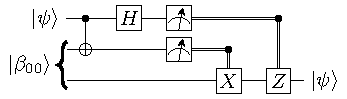
\includegraphics{teleport.pdf}

    Draw examples from Nielsen and Chuang, and the general literature.

 Simply change (if (condition) (branch) (branch))
 into
 ``
 Condition
 Measure []
 Jump label
 branch
 branch etc
 ``
 
 Curry also supports variable naming, blocks of qubits, classical callbacks, imports, \dots
 Curry can be called as a library and operated from python
 
 There are some easy targets for providing abstraction: common things like functions, conditionals, loops, integer data types, and so on. 
 However, let's jump into the quantum/probabilistic side of things.
 
 Models will fundamentally be composed of, generally, wave functions: Superpositions over all possible states.
 First, consider modeling a classical distribution. 
 We can successfully produce sampleable classical distributions on a quantum computer.
 For instance, consider the following model from the Church programming language tutorial.
 This code is specifying a probabilistic grammar for simple sentences about cooking.
 
 ```scheme
 (define (transition nonterminal)
   (case nonterminal
         (('D) (multinomial(list (list (terminal 'the))
                                 (list (terminal 'a)))
                           (list (/ 1 2) (/ 1 2))))
         (('N) (multinomial (list (list (terminal 'chef))
                                  (list (terminal 'soup))
                                  (list (terminal 'omelet)))
                            (list (/ 1 3) (/ 1 3) (/ 1 3))))
         (('V) (multinomial (list (list (terminal 'cooks))
                                  (list (terminal 'works)))
                            (list (/ 1 2) (/ 1 2))))
         (('A) (multinomial (list (list (terminal 'diligently)))
                            (list (/ 1 1))))
         (('AP) (multinomial (list (list 'A))
                             (list (/ 1 1))))
         (('NP) (multinomial (list (list 'D 'N))
                             (list (/ 1 1))))
         (('VP) (multinomial (list (list 'V 'AP)
                                   (list 'V 'NP))
                             (list (/ 1 2) (/ 1 2))))
         (('S) (multinomial (list (list 'NP 'VP))
                            (list (/ 1 1))))
         (else 'error)))
 ```
 
 More succinctly, this is specifying the following (toy) language model:
 ```scheme
 D(eterminer):      (uniform 'the' 'a')
 N(oun):            (uniform 'chef' 'omelet' 'soup')
 V(erb):            (uniform 'cooks' 'works')
 A(dverb):          (uniform 'diligently')
 AP(Adverb Phrase): (uniform A)
 NP(Noun Phrase):   (D, N)
 VP(Verb Phrase):   (uniform (V AP) (V NP))
 S(entence):        (NP, VP)
 ```
 
 To make things even simpler, let's first just consider modeling a randomly sampled Noun-Phrase (which is the first part in sampling a full toy sentence).
 The noun-phrase is a concatenation of a determiner and a noun. In our toy example, we have two determiners and three nouns, both uniformly sampled, which makes for a total of six options with equal probability.
 So, we'll need three qubits to model this. Curry has builtins for these distributions.
 ```scheme
 (def determiner-qubit 0)
 (def noun-qubits 1 2)
 (bernoulli 0.5 determiner-qubit)
 (multinomial 0.33 0.33 0.34 noun-qubits)
 ```
 
 The output is the following (using a local simulator):
 ```
 grid {curry}: ./compile examples/test.lisp
 
 [['def', 'determiner-qubit', '0'],
  ['def', 'noun-qubits', '1', '2'],
  ['bernoulli', '0.5', 'determiner-qubit'],
  ['multinomial', '0.33', '0.33', '0.34', 'noun-qubits']]
 
 {'000': 0.17, '001': 0.16, '010': 0.17, '011': 0.17, '100': 0.16, '101': 0.16}
 
 277.4035930633545 ms simulated runtime
 ```
 
 In our output, the rightmost bit is representing the determiner, and the other two bits are representing the noun.
 So the output is:
 ```python3
 {'the chef' : 1/6, 'a chef' : 1/6, 'the omelet' : 1/6, 'a omelet' : 1/6, 'the soup' : 1/6, 'a soup' : 1/6}
 ```
 Now, let's consider the rest of the model.
 When we sample a Verb Phrase, it contains recursive elements.
 So, it will branch (with equal probabilities) to either (V AP) or (V NP).
 Before diving in, let's look at branching in quantum computers.
 
 Consider preparing a bell state:
 ```
 (h 0)
 (cnot 0 1)
 ```
 And distinguish this from the following, which will produce the same classical measurements, but no entanglement (because the state of the first qubit is known before producing the state in the second qubit). 
 In this case, the state 01 is possible, because the first qubit may be measured in the 1 state, and the second qubit is unprepared, and in the zero state.
 ```
 (bernoulli 0.5 0)
 (measure 0 0)
 (if 0 (x 1) (nop))
 ```
 
 So, when creating a probabilistic model which branches, we distinguish between these two types of branching, because only one truly creates an entangled state.
 However, this makes representing information slightly more difficult, because we will not know which bits correspond to which states (unless we encode this, which we will).

\section{Conclusion}

In the creation of a Qurry and its corresponding framework, it is hoped that this will aid the development of quantum algorithms, as algorithm designers will have a new, richer, more abstract vocabulary with which to express themselves.
To recap, this goal is approached in the following N ways.
By introduction of lightweight abstractions from the C++ school of thought, efficient and transparent programming interfaces are created.
Through specialized libraries, Qurry can claim to be a generalized library, while still offering powerful sub-frameworks for specific tasks.
With functional programming paradigms, Qurry can move towards higher levels of abstraction as the semantics of quantum programming become better understood.
Lastly, by creating a rapid prototyping framework, new language features can be developed in a bottom-up style, which will allow Qurry to be created naturally, instead of artificially.


 \appendices
 \section{Appendix one}
Appendix content

% use section* for acknowledgment
\section*{Acknowledgment}

The author would like to thank Dr. Will Zeng of Rigetti computing, an organizer of the Unitary Fund, Dr. Ajay Bansal of Arizona State University, PLoS and other donators to the unitary fund, and ASU's FURI program.

% Can use something like this to put references on a page
% by themselves when using endfloat and the captionsoff option.
\ifCLASSOPTIONcaptionsoff
  \newpage
\fi

% trigger a \newpage just before the given reference
% number - used to balance the columns on the last page
% adjust value as needed - may need to be readjusted if
% the document is modified later
%\IEEEtriggeratref{8}
% The "triggered" command can be changed if desired:
%\IEEEtriggercmd{\enlargethispage{-5in}}

% references section

% can use a bibliography generated by BibTeX as a .bbl file
% BibTeX documentation can be easily obtained at:
% http://mirror.ctan.org/biblio/bibtex/contrib/doc/
% The IEEEtran BibTeX style support page is at:
% http://www.michaelshell.org/tex/ieeetran/bibtex/
%\bibliographystyle{IEEEtran}
% argument is your BibTeX string definitions and bibliography database(s)
%\bibliography{IEEEabrv,../bib/paper}
%
% <OR> manually copy in the resultant .bbl file
% set second argument of \begin to the number of references
% (used to reserve space for the reference number labels box)

\begin{thebibliography}{1}

\bibitem{IEEEhowto:kopka}
H.~Kopka and P.~W. Daly, \emph{A Guide to \LaTeX}, 3rd~ed.\hskip 1em plus
  0.5em minus 0.4em\relax Harlow, England: Addison-Wesley, 1999.

\end{thebibliography}

\begin{IEEEbiographynophoto}{Lucas Saldyt}
    is currently a student researcher at Arizona State University, and has previously worked for Sandia National Laboratories and Los Alamos National Laboratories as a student intern in the quantum computing department.
\end{IEEEbiographynophoto}

\end{document}
